\documentclass[]{article}
\usepackage{amsmath}
\usepackage{amsfonts}
\usepackage{amssymb}
\usepackage{amsthm}
\usepackage{cancel}
\usepackage{graphicx}
\usepackage{pgfplots}
\usepackage{pdfpages}
\usepackage{hyperref}

\renewcommand{\thesection}{\arabic{section}}
\renewcommand{\thesubsection}{\thesection.\alph{subsection}}
\renewcommand{\thesubsubsection}{\thesubsection.\roman{subsubsection}}

\newcommand{\iprod}[2]{\left\langle #1, #2 \right\rangle}
\renewcommand{\vec}[1]{\mathbf{#1}}
\newcommand{\corr}{\operatorname{corr}}

\newtheorem{genthm}{Theorem}

%opening
\title{EECS 16A HW12}
\author{Bryan Ngo}
\date{2019-11-20}

\begin{document}

\maketitle

\section{Op Amp with Output Current}

\subsection{}

There are three equations that we concern ourselves with: 
\begin{align}
	V_{out} &= A(V_{\text{ref}} - V^-) \\
	V^- &= I_O R \\
	V^- &= V_{out} - \frac{I_O}{g_{ms}}
\end{align}
setting (2) and (3) equal and plugging in (1), 
\begin{align}
	I_O R &= A V_{\text{ref}} - A I_O R - \frac{I_O}{g_{ms}} \\
	I_O \left(R + AR + \frac{1}{g_{ms}}\right) &= A V_{\text{ref}} \\
	I_O &= \frac{AV_{\text{ref}}}{R + AR + \frac{1}{g_{ms}}}
\end{align}
Since there is no expression for \(R_L\) in the answer, the current is independent of \(R_L\). 

\subsection{}

The circuit is considered a voltage-controlled current source. 

\section{Cauchy-Schwarz Inequality}

\subsection{}

\begin{align}
	||\vec{v}|| &= \sqrt{\iprod{\vec{v}}{\vec{v}}} = \sqrt{r^2 \cos^2(\theta) + r^2 \sin^2(\theta)} = r\cancelto{1}{\sqrt{\cos^2(\theta) + \sin^2(\theta)}} = r \\
	||\vec{w}|| &= \sqrt{\iprod{\vec{w}}{\vec{w}}} = \sqrt{t^2 \cos^2(\phi) + t^2 \sin^2(\phi)} = t\cancelto{1}{\sqrt{\cos^2(\phi) + \sin^2(\phi)}} = t
\end{align}

\subsection{}

\begin{equation}
	\iprod{\vec{v}}{\vec{w}} = r t \cos(\theta) \cos(\phi) + r t \sin(\theta) \sin(\phi) = r t(\cos(\theta - \phi)) = ||\vec{v}|| ||\vec{w}|| \cos(\theta - \phi)
\end{equation}

\subsection{}

\begin{proof}
By definition of the cosine function, 
\begin{align}
	-1 \le \cos(\theta - \phi) &\le 1 \\
	(||\vec{v}|| ||\vec{w}||) \cdot -1 \le (||\vec{v}|| ||\vec{w}||) \cdot \cos(\theta - \phi) &\le (||\vec{v}|| ||\vec{w}||) \cdot 1 \\
	\operatorname{abs}(||\vec{v}|| ||\vec{w}|| \cos(\theta - \phi)) &\le ||\vec{v}|| ||\vec{w}|| \\
	|\iprod{\vec{v}}{\vec{w}}| &\le ||\vec{v}|| ||\vec{w}||
\end{align}
\end{proof}

\section{Mechanical Linear Correlation}

\stepcounter{subsection}

\subsection{}

\begin{flushleft}
\begin{tabular}{c|ccccccccccc}
	\(\vec{s}_1[n]\) & 0 & 0 & 0 & 2 & -2 & 2 & -2 & 0 & 0 & 0 \\
	\hline
	\(\vec{s}_2[n + 3]\) & 1 & 2 & 3 & 4 & 0 & 0 & 0 & 0 & 0 & 0 \\
	\hline
	\(\iprod{\vec{s}_1[n]}{\vec{s}_2[n + 3]}\) & 0 & 0 & 0 & 8 & 0 & 0 & 0 & 0 & 0 & 0 & \(= 8\) \\
\end{tabular} \vspace{5 mm}
\begin{tabular}{c|ccccccccccc}
	\(\vec{s}_1[n]\) & 0 & 0 & 0 & 2 & -2 & 2 & -2 & 0 & 0 & 0 \\
	\hline
	\(\vec{s}_2[n + 2]\) & 0 & 1 & 2 & 3 & 4 & 0 & 0 & 0 & 0 & 0 \\
	\hline
	\(\iprod{\vec{s}_1[n]}{\vec{s}_2[n + 2]}\) & 0 & 0 & 0 & 6 & -8 & 0 & 0 & 0 & 0 & 0 & \(= -2\) \\
\end{tabular} \vspace{5 mm}
\begin{tabular}{c|ccccccccccc}
	\(\vec{s}_1[n]\) & 0 & 0 & 0 & 2 & -2 & 2 & -2 & 0 & 0 & 0 \\
	\hline
	\(\vec{s}_2[n + 1]\) & 0 & 0 & 1 & 2 & 3 & 4 & 0 & 0 & 0 & 0 \\
	\hline
	\(\iprod{\vec{s}_1[n]}{\vec{s}_2[n + 1]}\) & 0 & 0 & 0 & 4 & -6 & 8 & 0 & 0 & 0 & 0 & \(= 6\) \\
\end{tabular} \vspace{5 mm}
\begin{tabular}{c|ccccccccccc}
	\(\vec{s}_1[n]\) & 0 & 0 & 0 & 2 & -2 & 2 & -2 & 0 & 0 & 0 \\
	\hline
	\(\vec{s}_2[n]\) & 0 & 0 & 0 & 1 & 2 & 3 & 4 & 0 & 0 & 0 \\
	\hline
	\(\iprod{\vec{s}_1[n]}{\vec{s}_2[n]}\) & 0 & 0 & 0 & 2 & -4 & 6 & -8 & 0 & 0 & 0 & \(= -4\) \\
\end{tabular} \vspace{5 mm}
\begin{tabular}{c|ccccccccccc}
	\(\vec{s}_1[n]\) & 0 & 0 & 0 & 2 & -2 & 2 & -2 & 0 & 0 & 0 \\
	\hline
	\(\vec{s}_2[n - 1]\) & 0 & 0 & 0 & 0 & 1 & 2 & 3 & 4 & 0 & 0 \\
	\hline
	\(\iprod{\vec{s}_1[n]}{\vec{s}_2[n - 1]}\) & 0 & 0 & 0 & 0 & -2 & 4 & -6 & 0 & 0 & 0 & \(= -4\) \\
\end{tabular} \vspace{5 mm}
\begin{tabular}{c|ccccccccccc}
	\(\vec{s}_1[n]\) & 0 & 0 & 0 & 2 & -2 & 2 & -2 & 0 & 0 & 0 \\
	\hline
	\(\vec{s}_2[n - 2]\) & 0 & 0 & 0 & 0 & 0 & 1 & 2 & 3 & 4 & 0 \\
	\hline
	\(\iprod{\vec{s}_1[n]}{\vec{s}_2[n - 2]}\) & 0 & 0 & 0 & 0 & 0 & 2 & -4 & 0 & 0 & 0 & \(= -2\) \\
\end{tabular} \vspace{5 mm}
\begin{tabular}{c|ccccccccccc}
	\(\vec{s}_1[n]\) & 0 & 0 & 0 & 2 & -2 & 2 & -2 & 0 & 0 & 0 \\
	\hline
	\(\vec{s}_2[n - 3]\) & 0 & 0 & 0 & 0 & 0 & 0 & 1 & 2 & 3 & 4 \\
	\hline
	\(\iprod{\vec{s}_1[n]}{\vec{s}_2[n - 3]}\) & 0 & 0 & 0 & 0 & 0 & 0 & -2 & 0 & 0 & 0 & \(= -2\) \\
\end{tabular} \vspace{5 mm}
\begin{tikzpicture}
	\begin{axis}[
	xmin=-4, xmax=4,
	ymin=-10, ymax=10
	]
	\addplot [ycomb,color=blue,mark=*,thick] coordinates {(-3,8) (-2,-2) (-1,6) (0,-4) (1,-4) (2,-2) (3,-2)};
	\addplot [color=black,thick] coordinates {(-3,0) (3,0)};
	\end{axis}
\end{tikzpicture}
\end{flushleft}

\subsection{}

The iPython notebook tells us that when the vectors correlated switch spots, the entire graph flips. This tells us that
\begin{equation}
	\corr_{\vec{s}_1}(\vec{s}_2)[k] = \corr_{\vec{s}_2}(\vec{s}_1)[-k]
\end{equation}

\stepcounter{subsection}
\stepcounter{subsection}

\section{Audio File Matching}

\subsection{}

If \(\vec{x}_1 = \vec{x}_2\), 
\begin{equation}
	\iprod{\vec{x}_1}{\vec{x}_2} = \iprod{\vec{x}_1}{\vec{x}_1} = ||\vec{x}_1||^2 = \underbrace{1^2 + 1^2 + \cdots}_{N \text{ times}} = N
\end{equation}
In the second case, 
\begin{equation}
	\iprod{\vec{x}_1}{\vec{x}_2} = 1(1) + 1(-1) + \cdots = 0
\end{equation}
This only works when \(N\) is even because then there are as many negatives as there are positives so it cancels out. 
We can use the inner product to determine the similarity of two vectors, since geometrically it gives us a measure of how "parallel" two vectors are. 

\subsection{}

Finding \(\corr_{\vec{x}}(\vec{y}_1[k])\), 

\begin{flushleft}
\begin{tabular}{c|ccccccccccccc}
	\(\vec{x}[n]\) & 0 & 0 & -1 & 1 & 1 & -1 & 1 & 1 & -1 & 1 & 0 & 0 \\
	\hline
	\(\vec{y}_1[n + 2]\) & 1 & 1 & 1 & 0 & 0 & 0 & 0 & 0 & 0 & 0 & 0 & 0 \\
	\(\corr_{\vec{x}}(\vec{y}_1[-2])\) & 0 & 0 & 1 & 0 & 0 & 0 & 0 & 0 & 0 & 0 & 0 & 0 & \(= 1\) \\
\end{tabular} \vspace{5 mm}
\begin{tabular}{c|ccccccccccccc}
	\(\vec{x}[n]\) & 0 & 0 & -1 & 1 & 1 & -1 & 1 & 1 & -1 & 1 & 0 & 0 \\
	\hline
	\(\vec{y}_1[n + 1]\) & 0 & 1 & 1 & 1 & 0 & 0 & 0 & 0 & 0 & 0 & 0 & 0 \\
	\(\corr_{\vec{x}}(\vec{y}_1[-1])\) & 0 & 0 & -1 & -1 & 0 & 0 & 0 & 0 & 0 & 0 & 0 & 0 & \(= -2\) \\
\end{tabular} \vspace{5 mm}
\begin{tabular}{c|ccccccccccccc}
	\(\vec{x}[n]\) & 0 & 0 & -1 & 1 & 1 & -1 & 1 & 1 & -1 & 1 & 0 & 0 \\
	\hline
	\(\vec{y}_1[n]\) & 0 & 0 & 1 & 1 & 1 & 0 & 0 & 0 & 0 & 0 & 0 & 0 \\
	\(\corr_{\vec{x}}(\vec{y}_1[0])\) & 0 & 0 & -1 & 1 & -1 & 0 & 0 & 0 & 0 & 0 & 0 & 0 & \(= -1\) \\
\end{tabular} \vspace{5 mm}
\begin{tabular}{c|ccccccccccccc}
	\(\vec{x}[n]\) & 0 & 0 & -1 & 1 & 1 & -1 & 1 & 1 & -1 & 1 & 0 & 0 \\
	\hline
	\(\vec{y}_1[n - 1]\) & 0 & 0 & 0 & 1 & 1 & 1 & 0 & 0 & 0 & 0 & 0 & 0 \\
	\(\corr_{\vec{x}}(\vec{y}_1[1])\) & 0 & 0 & 0 & 1 & 1 & 1 & 0 & 0 & 0 & 0 & 0 & 0 & \(= 3\) \\
\end{tabular} \vspace{5 mm}
\begin{tabular}{c|ccccccccccccc}
	\(\vec{x}[n]\) & 0 & 0 & -1 & 1 & 1 & -1 & 1 & 1 & -1 & 1 & 0 & 0 \\
	\hline
	\(\vec{y}_1[n - 2]\) & 0 & 0 & 0 & 0 & 1 & 1 & 1 & 0 & 0 & 0 & 0 & 0 \\
	\(\corr_{\vec{x}}(\vec{y}_1[2])\) & 0 & 0 & 0 & 0 & 1 & -1 & -1 & 0 & 0 & 0 & 0 & 0 & \(= -2\) \\
\end{tabular} \vspace{5 mm}
\begin{tabular}{c|ccccccccccccc}
	\(\vec{x}[n]\) & 0 & 0 & -1 & 1 & 1 & -1 & 1 & 1 & -1 & 1 & 0 & 0 \\
	\hline
	\(\vec{y}_1[n - 3]\) & 0 & 0 & 0 & 0 & 0 & 1 & 1 & 1 & 0 & 0 & 0 & 0 \\
	\(\corr_{\vec{x}}(\vec{y}_1[3])\) & 0 & 0 & 0 & 0 & 0 & -1 & 1 & -1 & 0 & 0 & 0 & 0 & \(= -2\) \\
\end{tabular} \vspace{5 mm}
\begin{tabular}{c|ccccccccccccc}
	\(\vec{x}[n]\) & 0 & 0 & -1 & 1 & 1 & -1 & 1 & 1 & -1 & 1 & 0 & 0 \\
	\hline
	\(\vec{y}_1[n - 4]\) & 0 & 0 & 0 & 0 & 0 & 0 & 1 & 1 & 1 & 0 & 0 & 0 \\
	\(\corr_{\vec{x}}(\vec{y}_1[4])\) & 0 & 0 & 0 & 0 & 0 & 0 & 1 & 1 & 1 & 0 & 0 & 0 & \(= 3\) \\
\end{tabular} \vspace{5 mm}
\begin{tabular}{c|ccccccccccccc}
	\(\vec{x}[n]\) & 0 & 0 & -1 & 1 & 1 & -1 & 1 & 1 & -1 & 1 & 0 & 0 \\
	\hline
	\(\vec{y}_1[n - 5]\) & 0 & 0 & 0 & 0 & 0 & 0 & 0 & 1 & 1 & 1 & 0 & 0 \\
	\(\corr_{\vec{x}}(\vec{y}_1[5])\) & 0 & 0 & 0 & 0 & 0 & 0 & 0 & 1 & -1 & -1 & 0 & 0 & \(= -2\) \\
\end{tabular} \vspace{5 mm}
\begin{tabular}{c|ccccccccccccc}
	\(\vec{x}[n]\) & 0 & 0 & -1 & 1 & 1 & -1 & 1 & 1 & -1 & 1 & 0 & 0 \\
	\hline
	\(\vec{y}_1[n - 6]\) & 0 & 0 & 0 & 0 & 0 & 0 & 0 & 0 & 1 & 1 & 1 & 0 \\
	\(\corr_{\vec{x}}(\vec{y}_1[6])\) & 0 & 0 & 0 & 0 & 0 & 0 & 0 & 0 & -1 & 1 & 0 & 0 & \(= 0\) \\
\end{tabular} \vspace{5 mm}
\begin{tabular}{c|ccccccccccccc}
	\(\vec{x}[n]\) & 0 & 0 & -1 & 1 & 1 & -1 & 1 & 1 & -1 & 1 & 0 & 0 \\
	\hline
	\(\vec{y}_1[n - 7]\) & 0 & 0 & 0 & 0 & 0 & 0 & 0 & 0 & 0 & 1 & 1 & 1 & 0 \\
	\(\corr_{\vec{x}}(\vec{y}_1[7])\) & 0 & 0 & 0 & 0 & 0 & 0 & 0 & 0 & 0 & 1 & 0 & 0 & \(= 1\) \\
\end{tabular} \vspace{5 mm}
\end{flushleft}

Here we find \(\max\{\corr_{\vec{x}}(\vec{y}_1[k])\} = 3\) at \(k = 1, 4\). For \(\vec{y}_2\), 

\begin{flushleft}
\begin{tabular}{c|ccccccccccccc}
	\(\vec{x}[n]\) & 0 & 0 & -1 & 1 & 1 & -1 & 1 & 1 & -1 & 1 & 0 & 0 \\
	\hline
	\(\vec{y}[n + 2]\) & 1 & 1 & 1 & 0 & 0 & 0 & 0 & 0 & 0 & 0 & 0 & 0 \\
	\(\corr_{\vec{x}}(\vec{y}_1[-2])\) & 0 & 0 & -1 & 0 & 0 & 0 & 0 & 0 & 0 & 0 & 0 & 0 & \(= -1\) \\
\end{tabular} \vspace{5 mm}
\begin{tabular}{c|ccccccccccccc}
	\(\vec{x}[n]\) & 0 & 0 & -1 & 1 & 1 & -1 & 1 & 1 & -1 & 1 & 0 & 0 \\
	\hline
	\(\vec{y}_1[n + 1]\) & 0 & 1 & 1 & 1 & 0 & 0 & 0 & 0 & 0 & 0 & 0 & 0 \\
	\(\corr_{\vec{x}}(\vec{y}_1[-1])\) & 0 & 0 & -1 & 1 & 0 & 0 & 0 & 0 & 0 & 0 & 0 & 0 & \(= 0\) \\
\end{tabular} \vspace{5 mm}
\begin{tabular}{c|ccccccccccccc}
	\(\vec{x}[n]\) & 0 & 0 & -1 & 1 & 1 & -1 & 1 & 1 & -1 & 1 & 0 & 0 \\
	\hline
	\(\vec{y}_1[n]\) & 0 & 0 & 1 & 1 & 1 & 0 & 0 & 0 & 0 & 0 & 0 & 0 \\
	\(\corr_{\vec{x}}(\vec{y}_1[0])\) & 0 & 0 & -1 & 1 & 1 & 0 & 0 & 0 & 0 & 0 & 0 & 0 & \(= 1\) \\
\end{tabular} \vspace{5 mm}
\begin{tabular}{c|ccccccccccccc}
	\(\vec{x}[n]\) & 0 & 0 & -1 & 1 & 1 & -1 & 1 & 1 & -1 & 1 & 0 & 0 \\
	\hline
	\(\vec{y}_1[n - 1]\) & 0 & 0 & 0 & 1 & 1 & 1 & 0 & 0 & 0 & 0 & 0 & 0 \\
	\(\corr_{\vec{x}}(\vec{y}_1[1])\) & 0 & 0 & 0 & 1 & 1 & -1 & 0 & 0 & 0 & 0 & 0 & 0 & \(= 1\) \\
\end{tabular} \vspace{5 mm}
\begin{tabular}{c|ccccccccccccc}
	\(\vec{x}[n]\) & 0 & 0 & -1 & 1 & 1 & -1 & 1 & 1 & -1 & 1 & 0 & 0 \\
	\hline
	\(\vec{y}_1[n - 2]\) & 0 & 0 & 0 & 0 & 1 & 1 & 1 & 0 & 0 & 0 & 0 & 0 \\
	\(\corr_{\vec{x}}(\vec{y}_1[2])\) & 0 & 0 & 0 & 0 & 1 & -1 & 1 & 0 & 0 & 0 & 0 & 0 & \(= 1\) \\
\end{tabular} \vspace{5 mm}
\begin{tabular}{c|ccccccccccccc}
	\(\vec{x}[n]\) & 0 & 0 & -1 & 1 & 1 & -1 & 1 & 1 & -1 & 1 & 0 & 0 \\
	\hline
	\(\vec{y}_1[n - 3]\) & 0 & 0 & 0 & 0 & 0 & 1 & 1 & 1 & 0 & 0 & 0 & 0 \\
	\(\corr_{\vec{x}}({\vec{y}_1}[3])\) & 0 & 0 & 0 & 0 & 0 & -1 & 1 & 1 & 0 & 0 & 0 & 0 & \(= 1\) \\
\end{tabular} \vspace{5 mm}
\begin{tabular}{c|ccccccccccccc}
	\(\vec{x}[n]\) & 0 & 0 & -1 & 1 & 1 & -1 & 1 & 1 & -1 & 1 & 0 & 0 \\
	\hline
	\(\vec{y}_1[n - 4]\) & 0 & 0 & 0 & 0 & 0 & 0 & 1 & 1 & 1 & 0 & 0 & 0 \\
	\(\corr_{\vec{x}}(\vec{y}_1[4])\) & 0 & 0 & 0 & 0 & 0 & 0 & 1 & 1 & -1 & 0 & 0 & 0 & \(= 1\) \\
\end{tabular} \vspace{5 mm}
\begin{tabular}{c|ccccccccccccc}
	\(\vec{x}[n]\) & 0 & 0 & -1 & 1 & 1 & -1 & 1 & 1 & -1 & 1 & 0 & 0 \\
	\hline
	\(\vec{y}_1[n - 5]\) & 0 & 0 & 0 & 0 & 0 & 0 & 0 & 1 & 1 & 1 & 0 & 0 \\
	\(\corr_{\vec{x}}(\vec{y}_1[5])\) & 0 & 0 & 0 & 0 & 0 & 0 & 0 & 1 & -1 & 1 & 0 & 0 & \(= 1\) \\
\end{tabular} \vspace{5 mm}
\begin{tabular}{c|ccccccccccccc}
	\(\vec{x}[n]\) & 0 & 0 & -1 & 1 & 1 & -1 & 1 & 1 & -1 & 1 & 0 & 0 \\
	\hline
	\(\vec{y}_1[n - 6]\) & 0 & 0 & 0 & 0 & 0 & 0 & 0 & 0 & 1 & 1 & 1 & 0 \\
	\(\corr_{\vec{x}}(\vec{y}_1[6])\) & 0 & 0 & 0 & 0 & 0 & 0 & 0 & 0 & -1 & 1 & 0 & 0 & \(= 0\) \\
\end{tabular} \vspace{5 mm}
\begin{tabular}{c|ccccccccccccc}
	\(\vec{x}[n]\) & 0 & 0 & -1 & 1 & 1 & -1 & 1 & 1 & -1 & 1 & 0 & 0 \\
	\hline
	\(\vec{y}_1[n - 7]\) & 0 & 0 & 0 & 0 & 0 & 0 & 0 & 0 & 0 & 1 & 1 & 1 \\
	\(\corr_{\vec{x}}(\vec{y}_1[7])\) & 0 & 0 & 0 & 0 & 0 & 0 & 0 & 0 & 0 & 1 & 0 & 0 & \(= 1\) \\
\end{tabular} \vspace{5 mm}
\end{flushleft}

Here we find \(\max\{\corr_{\vec{x}}(\vec{y}_1[k])\} = 1\) at \(k \in [0, 5]\). 

\subsection{}

We will expect a correlation peak at \(k = 4\), as you will get
\begin{equation}
	\iprod{\vec{x}}{\vec{y}[4]} = 2 \cdot 1 + 2 \cdot 2 + 3 \cdot 3 = 15
\end{equation}
which is clearly what is not intended, since although the magnitudes are highest here, that does not necessarily mean the pitches, or directions,  line up.

\stepcounter{subsection}
\stepcounter{subsection}

\section{GPS Receivers}

\subsection{}

We observe that there is a relatively low correlation until the gold code matches with itself at offset zero, at which point a large spike of 1023 is observed, confirming a high auto-correlation. 

\subsection{}

We observe a very low correlation between satellite 13 and satellite 10, with a peak of about 80. 

\subsection{}

We notice that even noise yields a very low correlation between it and satellite 10, with a max correlation of only about 100. 

\subsection{}

We notice that even \emph{Gaussian} noise yields a very low correlation between it and satellite 10, with a max correlation of only about 100. 

\subsection{}

We find peaks for \texttt{signal1} at Satellites \(\{4, 7, 13, 19\}\). 

\subsection{}

Satellite 3 emits a signal \(\{1, -1, -1, -1, 1\}\). 

\subsection{}

Satellite 5 has a delay of 0, and Satellite 20 has a delay of +506. 

\section{\textit{Gold}en Positioning System}

\subsection{}

The satellite is transmitting the message \(\{1, -1, -1, 1\}\). 

\subsection{}

\begin{center}
\begin{tabular}{c|ccccccccccccc}
	\(\vec{r}\) & 0 & 1 & 1 & -1 & 1 & -1 & -1 & -1 & 1 & -1 & 1 & 0 \\
	\hline
	\(\vec{g}[n + 1]\) & 1 & 1 & -1 & 1 & -1 & 0 & 0 & 0 & 0 & 0 & 0 & 0 \\
	\hline
	\(\corr_{\vec{r}}(\vec{g})[-1]\) & 0 & 1 & -1 & -1 & -1 & 0 & 0 & 0 & 0 & 0 & 0 & 0 & \(= -2\) \\
\end{tabular} \vspace{5 mm}
\begin{tabular}{c|ccccccccccccc}
	\(\vec{r}\) & 0 & 1 & 1 & -1 & 1 & -1 & -1 & -1 & 1 & -1 & 1 & 0 \\
	\hline
	\(\vec{g}[n]\) & 0 & 1 & 1 & -1 & 1 & -1 & 0 & 0 & 0 & 0 & 0 & 0 \\
	\hline
	\(\corr_{\vec{r}}(\vec{g})[0]\) & 0 & 1 & 1 & 1 & 1 & 1 & 0 & 0 & 0 & 0 & 0 & 0 & \(= 5\) \\
\end{tabular} \vspace{5 mm}
\begin{tabular}{c|ccccccccccccc}
	\(\vec{r}\) & 0 & 1 & 1 & -1 & 1 & -1 & -1 & -1 & 1 & -1 & 1 & 0 \\
	\hline
	\(\vec{g}[n - 1]\) & 0 & 0 & 1 & 1 & -1 & 1 & -1 & 0 & 0 & 0 & 0 & 0 \\
	\hline
	\(\corr_{\vec{r}}(\vec{g})[1]\) & 0 & 0 & 1 & -1 & -1 & -1 & 1 & 0 & 0 & 0 & 0 & 0 & \(= -1\) \\
\end{tabular} \vspace{5 mm}
\begin{tabular}{c|ccccccccccccc}
	\(\vec{r}\) & 0 & 1 & 1 & -1 & 1 & -1 & -1 & -1 & 1 & -1 & 1 & 0 \\
	\hline
	\(\vec{g}[n - 2]\) & 0 & 0 & 1 & 1 & -1 & 1 & -1 & 0 & 0 & 0 & 0 & 0 \\
	\hline
	\(\corr_{\vec{r}}(\vec{g})[2]\) & 0 & 0 & 1 & -1 & -1 & -1 & 1 & 0 & 0 & 0 & 0 & 0 & \(= -1\) \\
\end{tabular} \vspace{5 mm}
\begin{tabular}{c|ccccccccccccc}
	\(\vec{r}\) & 0 & 1 & 1 & -1 & 1 & -1 & -1 & -1 & 1 & -1 & 1 & 0 \\
	\hline
	\(\vec{g}[n - 3]\) & 0 & 0 & 0 & 1 & 1 & -1 & 1 & -1 & 0 & 0 & 0 & 0 \\
	\hline
	\(\corr_{\vec{r}}(\vec{g})[3]\) & 0 & 0 & 0 & -1 & 1 & 1 & -1 & 1 & 0 & 0 & 0 & 0 & \(= 1\) \\
\end{tabular} \vspace{5 mm}
\begin{tabular}{c|ccccccccccccc}
	\(\vec{r}\) & 0 & 1 & 1 & -1 & 1 & -1 & -1 & -1 & 1 & -1 & 1 & 0 \\
	\hline
	\(\vec{g}[n - 4]\) & 0 & 0 & 0 & 0 & 1 & 1 & -1 & 1 & -1 & 0 & 0 & 0 \\
	\hline
	\(\corr_{\vec{r}}(\vec{g})[4]\) & 0 & 0 & 0 & 0 & 1 & -1 & 1 & -1 & -1 & 0 & 0 & 0 & \(= -1\) \\
\end{tabular} \vspace{5 mm}
\begin{tabular}{c|ccccccccccccc}
	\(\vec{r}\) & 0 & 1 & 1 & -1 & 1 & -1 & -1 & -1 & 1 & -1 & 1 & 0 \\
	\hline
	\(\vec{g}[n - 5]\) & 0 & 0 & 0 & 0 & 0 & 1 & 1 & -1 & 1 & -1 & 0 & 0 \\
	\hline
	\(\corr_{\vec{r}}(\vec{g})[5]\) & 0 & 0 & 0 & 0 & 0 & -1 & -1 & 1 & 1 & 1 & 0 & 0 & \(= 1\) \\
\end{tabular} \vspace{5 mm}
\begin{tabular}{c|ccccccccccccc}
	\(\vec{r}\) & 0 & 1 & 1 & -1 & 1 & -1 & -1 & -1 & 1 & -1 & 1 & 0 \\
	\hline
	\(\vec{g}[n - 6]\) & 0 & 0 & 0 & 0 & 0 & 0 & 1 & 1 & -1 & 1 & -1 & 0 \\
	\hline
	\(\corr_{\vec{r}}(\vec{g})[6]\) & 0 & 0 & 0 & 0 & 0 & 0 & -1 & -1 & -1 & -1 & -1 & 0 & \(= -5\) \\
\end{tabular} \vspace{5 mm}
\begin{tabular}{c|ccccccccccccc}
	\(\vec{r}\) & 0 & 1 & 1 & -1 & 1 & -1 & -1 & -1 & 1 & -1 & 1 & 0 \\
	\hline
	\(\vec{g}[n - 7]\) &  0& 0 & 0 & 0 & 0 & 0 & 0 & 1 & 1 & -1 & 1 & -1 \\
	\hline
	\(\corr_{\vec{r}}(\vec{g})[7]\) & 0 & 0 & 0 & 0 & 0 & 0 & 0 & -1 & 1 & 1 & 1 & 0 & \(= 2\) \\
\end{tabular} \vspace{5 mm}
\begin{tikzpicture}
	\begin{axis}[
	xmin=-2, xmax=8,
	ymin=-10, ymax=10
	]
	\addplot [ycomb,color=blue,mark=*,thick] coordinates {(-1,-2) (0,5) (1, -1) (2,-1) (3,1) (4,-1) (5,1) (6,-5) (7,2)};
	\addplot [color=black,thick] coordinates {(-2,0) (8,0)};
	\end{axis}
\end{tikzpicture}
\end{center}
The peaks show where the signals match up with the Gold code, and their sign represents the modulation, in this case \(\{1, -1\}\). 

\subsection{}

\begin{center}
	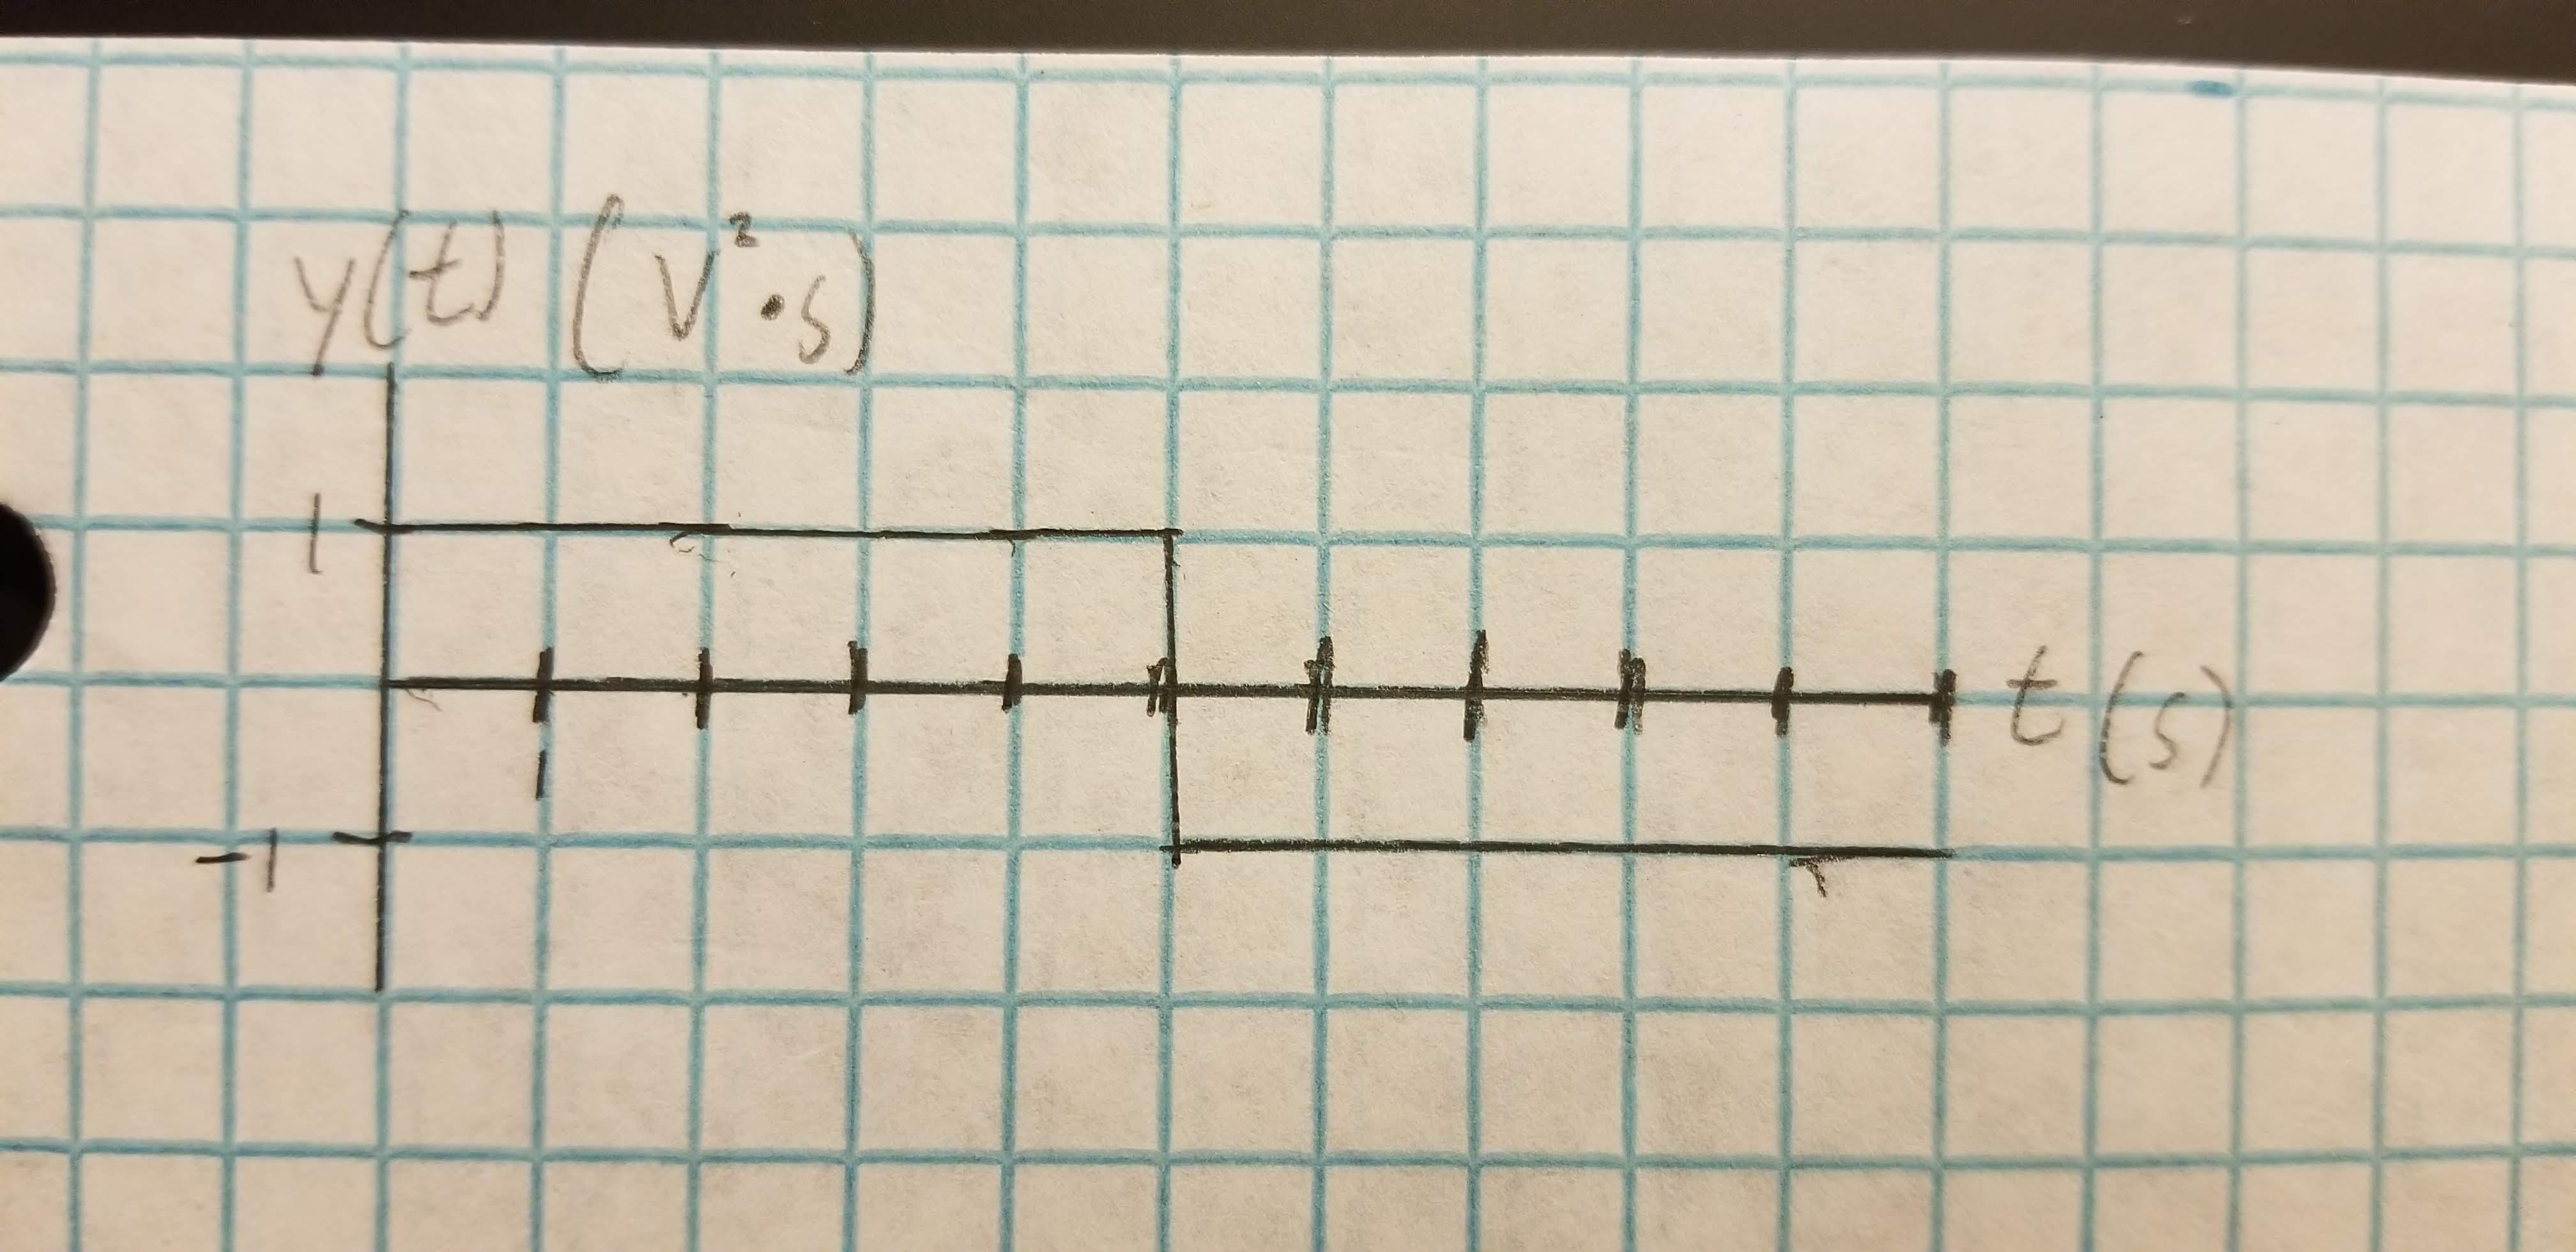
\includegraphics[width=0.7\linewidth]{20191122_024506}
\end{center}

\subsection{}

\begin{center}
	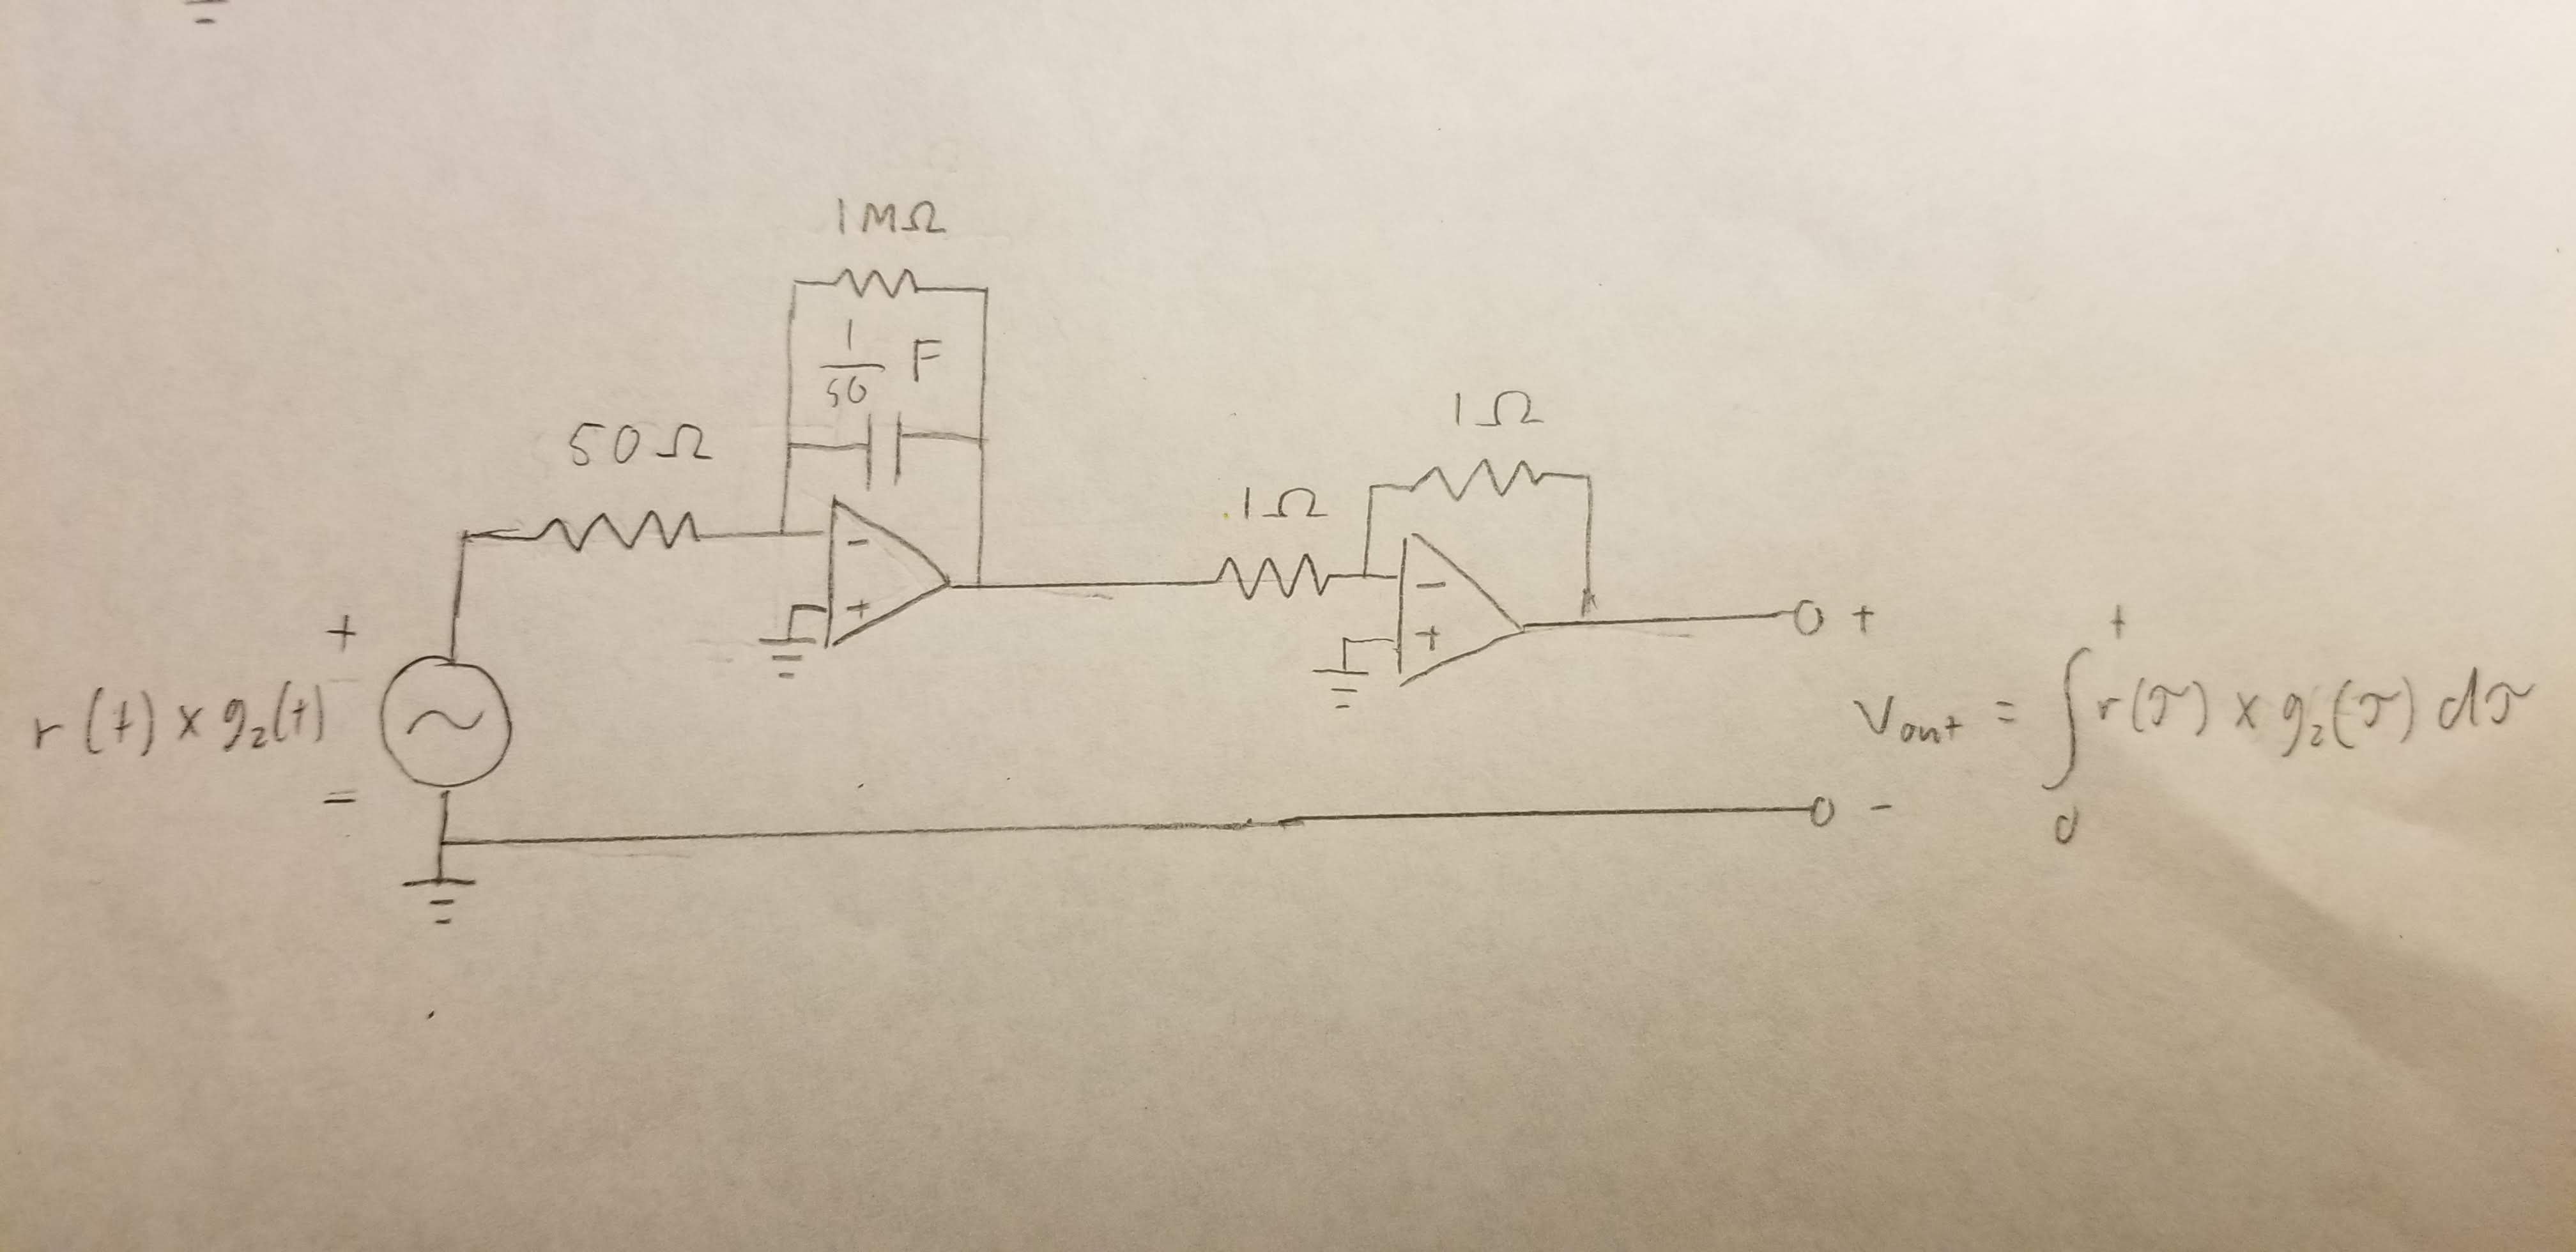
\includegraphics[width=0.7\linewidth]{20191122_024720}
\end{center}

\subsection{}

The equation for the distance is
\begin{equation}
	d_i = c (T_i - S_i)
\end{equation}

\subsection{}

\textbf{Four} satellites are needed in order to uniquely determine the position of the satellite in 3D space. 

\section{Homework Process and Study Group}

I did this homework by myself. 

\newpage

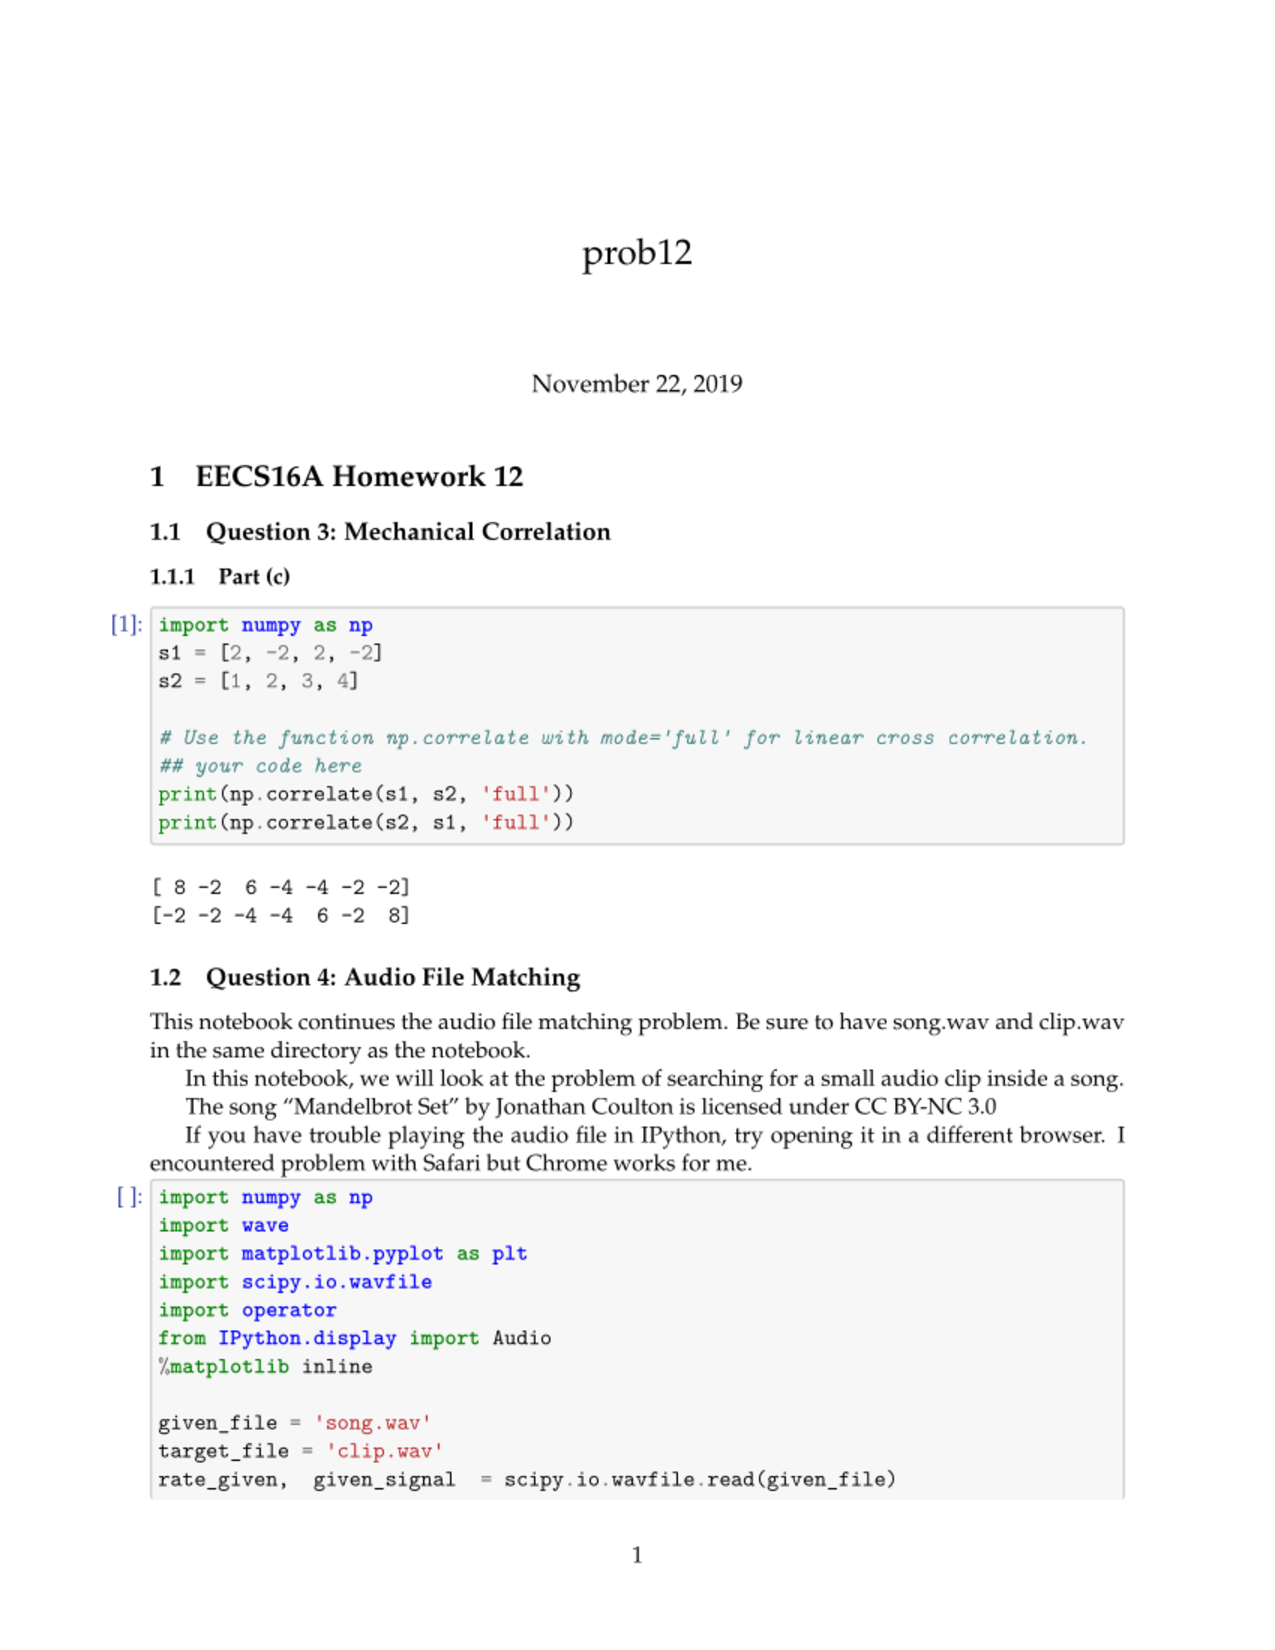
\includepdf[pages=-]{prob12.pdf}

\end{document}
